\section{Application-Specific RunTime Manager}
\label{sec:asrtm}


\begin{figure}
	\centering
	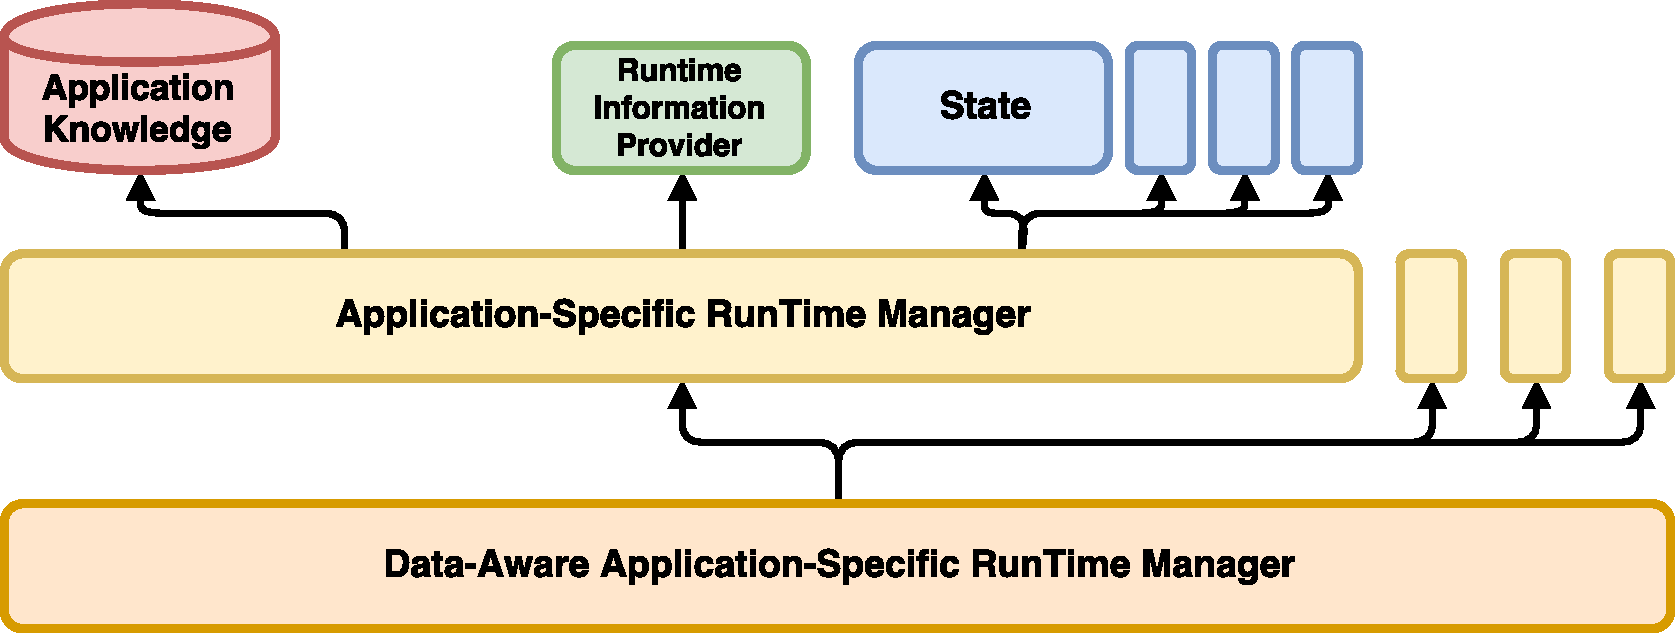
\includegraphics[scale=0.5]{asrtm}
	\caption{Overview of the manager module. }
	\label{fig:asrtm_module}
\end{figure}


This section describes the heart of mARGOt: the Manager module.
This module is in charge of selecting the most suitable configuration for the application.
\prettyref{fig:asrtm_module} shows the overall architecture of the module and the interaction between its principal elements.
In the remainder of the section, each element is explained in more details, following a bottom up approach.
However, the application developer has to interact only with the Application-Specific RunTime Manager (ASRTM) element or with the Data-Aware Application-Specific RunTime Manager element (DA-ASRTM).





\subsection{Rutime Information Provider}

This element relates the expected behavior of the application, in terms of EFPs, with the ones observed by the monitors.
In particular, since the framework will provide to the application a configuration which belong to the application knowledge, mARGOt knows the expected behavior of the application.
Therefore, if there is some difference between the expected behavior and the actual behavior of the application, the idea is that the framework must adjust the application knowledge accordingly.
To achieve this goal, the runtime information manage define the \textbf{coefficient error} $c_{e}^{i}$ for the \textit{i-th} field of the Operating Point as reported in \prettyref{eq:coefficient_error}.

\begin{equation}
\label{eq:coefficient_error}
c_{e}^{i}=\dfrac{expected_{i}}{mean_{i}}
\end{equation}

Where $mean_{i}$ represents the mean value observed by the related monitor and $expected_{i}$ represents the expected value, contained in the application knowledge.
Therefore, if $c_{e}^{i}$ is equal to $1$, it means that the $i-th$ field of the application knowledge matches perfectly with information provided by the monitor.
For numerical stability, if the observed value of the metric is exactly equal to zero, the framework adds a padding value of $1$ to the numerator and to the denominator.
In this case, $c_{e}^{i}$ tends to underestimate the actual value.

Typically, each measured value is affected by noise, produced either by the operating system or by the technique used to gather the measure.
To be robust with respect to this kind of noise, if the mean value observed by the monitor is within one standard deviation with respect to the expected mean value, we set $c_{e}^{i}$ equal to one.
The latter scenario requires that the target field is defined as a distribution in the application knowledge.
The idea is to adapt only if the difference is statistically significant.

Since some metrics may have spikes due to exceptional events, for instance when a process is migrated to another computing element, the runtime information provider store the last $n$ $c_{e}^{i}$ in a circular buffer, initially filled with ones (we assume that the application knowledge matches the reality).
The framework names \textbf{inertia} the value $n$.
If we set an high inertia to the \textit{i-th} field of an Operating Point, we are less prune to react over extraordinary events, but we are also less responsive in case of abrupt changes on the application behavior.
This parameter is exposed to the end user.


Therefore, the actual coefficient error used by the framework $\bar{c_{e}^{i}}$ is the average of all the $c_{e}^{i}$ gathered at runtime, as defined in \prettyref{eq:coefficient_error_real}.
Where $j$ indicates the \textit{j-th} $c_{e}^{i}$ in the circular buffer and $n$ indicates the inertia of the \textit{i-th} field.


\begin{equation}
\label{eq:coefficient_error_real}
\bar{c_{e}^{i}}=\dfrac{\sum_{j=0}^{n-1} c_{e,j}^{i}}{n}
\end{equation}


mARGOt uses $\bar{c_{e}^{i}}$ to perform a linear error propagation.
For examples, if with the selected configuration we expect a throughput of $10fps$, but the throughput monitor observe a throughput of $8fps$, mARGOt assumes that also all the other Operating Points will have a throughput that is $20\%$ slower than expected.
Since the error coefficient for the $i-th$ field of the Operating Point is computed in an independent way from the error coefficient of the $j-th$ field, mARGOt is able to perform a fine grained scaling of the application knowledge, to face changes in the execution environment.

From the integration point of view, the autotuner API enable the application developer to dynamically:
\begin{itemize}
	\item Relate a monitor to a field of the Operating Point.
	\item Remove all the information providers.
\end{itemize}






\subsection{State}

The application requirements are represented as a multi-objective constrained optimization problem.
Therefore, the autotuner is able to provide to the application the most suitable configuration, solving by inspection the optimization problem.
The state element is in charge of solving this problem, in en efficient way.
Let $ x = [x_1, \ldots, x_n] $ be the vector of the tunable parameters and $ p = [p_1, \ldots, p_n] $ the vector of the non-tunable parameters.
The tunable parameters are the software knobs that influence the application behavior, while the non-tunable parameters are the metric of interests, represented as distribution with a mean value and a standard deviation.
The constrained problem is described as in \prettyref{eq:optimization-general}.

\begin{equation}
\label{eq:optimization-general}
\begin{array}{rrclcl}
\displaystyle \max (\min) & \multicolumn{4}{l}{f(x;p)} \\
\textrm{s.t.} & C_1: \omega_1(x;p)  & \propto    & k_1  & with \quad \alpha_1 \quad confidence \\
&C_2: \omega_2(x;p)  & \propto   & k_2  &  \\
&C_3: \omega_3(x;p)  & \propto   & k_3  & with \quad \alpha_2 \quad confidence\\
& \ldots & & & \\
&C_n: \omega_n(x;p)  & \propto   & k_n
\end{array}
\end{equation}

In the description of the problem, $f$ denotes the objective function (named \textit{rank} in the autotuner context), which is defined as a composition of any of the variables defined in $x$ or $p$, using their mean values.
Let $C$ be the set of constraints, where each $C_i$ is a constraint expressed as the function $\omega_i$, defined over the tunable and non-tunable parameters, that must satisfy the relationship $ \propto  \in \{<,\leq ,> ,\geq \} $ with the threshold value $k_i$ and confidence $\alpha_i$ (if the parameter is a distribution).
Since we are agnostic about the distribution of the target parameter, the confidence is expressed as the number of times to consider its standard deviation.
These values are collected in a vector $ k= [ k_i ] $; together the vectors $p$ and $k$ are the input parameters of the problem.

If there is at least one configuration of the software knobs that satisfies the constraints, then the autotuner selects the one that maximize the value of the objective function.
Otherwise, the autotuner start to relax the constraints, starting from the ``least important'', to find the configuration closer to be valid.
For this reason, it is important to attach a \textit{priority} to each constraint, which is a numerical value that indicates how much important is a constraint.
Two constraints shall not have the same priority.
Moreover, it is not possible to express a constraint with $=$ sign, since in case mARGOt must relax the constraint, it is not possible to check if it is better to get a greater value or a lesser value.
In case the application user would like to express the $=$ relation, it must define two constraints ($\leq$ and $\geq$).
Since two constraints shall not have the same priority, mARGOt is able to tell in which direction is best to find the most suitable configuration, according to the priority of the constraints.

From the implementation point of view of the autotuner, a \textit{constraint} is defined against a \textit{goal} that state a single condition.
For example, $ C_1 $ is a \textit{constraint} that is defined by the \textit{goal} $ g_1 $.
The goal $ g_1 $ define the condition $ \omega_1(x;p) \propto k_1 $.
For this reason, declaring a new \textit{goal} $ goal_{new} $ does not change the optimization problem.
However, creating a \textit{constraint} that refers to the \textit{goal} $ goal_{new} $ does change the optimization problem.

Regarding the definition of the objective function, the framework exposes three ways of combine any variables defined in $x$ or $p$:
\begin{itemize}
	\item[Geometric] With this composition method, the objective function $f$ is defined as in \prettyref{eq:gemetric_combination},
		\begin{equation}
		\label{eq:gemetric_combination}
		f = \omega_1(x;p)^{c^1} \, \cdot \, \omega_2(x;p)^{c^2} \, \cdot \, \dots \, \cdot \, \omega_n(x;p)^{c^n}
		\end{equation}
		where the terms are multiplied by each other, using a user specified weights $c^1, c^2, \dots c^n$.
	\item[Linear] With this composition method, the objective function $f$ is defined as in \prettyref{eq:linear_combination},
		\begin{equation}
		\label{eq:linear_combination}
		f = \omega_1(x;p)\cdot{c^1}+\omega_2(x;p)\cdot{c^2}+\dots+\omega_n(x;p)\cdot{c^n}
		\end{equation}
		where the terms are added together, using a user specified weights $c^1, c^2, \dots c^n$.
	\item[Simple] With this composition method, the objective function $f$ is defined as the term $\omega_i(x;p)$
\end{itemize}

Since the time spent to solve the optimization problem is stolen from the application, the state element rearrange the application knowledge to minimize this overhead.
In particular, the introduced overhead is proportional to the amount of changes since the last time that the problem was solved.
Thus, if there are no changes, the time spent to solve the problem is negligible.


From the integration point of view, the autotuner API enable the application developer to dynamically:
\begin{itemize}
	\item Add/Remove a \textit{constraint}.
	\item Define the \textit{rank} function.
	\item Change the value of a \textit{goal}, thus on all the related \textit{constraints}.
\end{itemize}





\subsection{Application-Specific RunTime Manager}
	
This element orchestrates the application knowledge, the runtime information provider and the application states.
In fact, since the application might have different requirements according to the evolution of the system, it is possible to define several states.
Each state represents the multi-objective constrained optimization problem described in the previous section.

For the integration point of view, this element expose to the user a single interface to interact with Manager module of the framework.
In particular, the autotuner API enable the application developer to dynamically:
\begin{itemize}
	\item Add/Remove Operating Points
	\item Relate a monitor to a field of the Operating Point.
	\item Remove all the information providers.
	\item Create/Remove a state
	\item Select the active state
\end{itemize}
Those operations work at AS-RTM level, which means that are independent from the active state.
If you wold like to dynamically change the current active state, you might:
\begin{itemize}
	\item Set a different rank function
	\item Add/Remove a constraint
	\item Solve the optimization problem
	\item Get the most suitable configuration
\end{itemize}
If you want to change only the numerical value of a constraint, the application must change the value of the related goal instead.
Please, refer to the doxygen documentation for implementation details about the exposed API.


\subsection{Data-Aware Application-Specific RunTime Manager}

The AS-RTM assumes that the application behavior is either input independent or that there are few abrupt changes in the input, distributed over time.
Which means that the AS-RTM assumes either that the application EFPs depends only on the configuration of the software-knobs or that the adaptation due to the runtime information provider is enough to capture the relation between the EFPs of the application and the input data.

To overcome this limitation, mARGOt uses the Data-Aware AS-RTM (DA-ASRTM).
If the user is able to extract features of the input which are related to the behavior of the application, then it is possible to define the latter in terms of software knobs and data features.
In particular, the idea is to cluster the space of data features using the most representative cases and select, at run-time, the cluster closer to the actual input.


mARGOt represents each cluster of data feature with an AS-RTM.
This means that each cluster might have a different application knowledge, therefore the solution of the same optimization problem found by two different cluster, may be different.
For example, suppose that the input of the application kernel managed by mARGOt is a matrix, which must be elaborated.
Suppose also that the application kernel exposes a software knob that changes the precision of the elaboration and that the application user would like to maximize the quality of the elaboration given a time budget.
In this case we might use the size of the matrix as data feature, defining few clusters for the most representative sizes.
According to the application knowledge, a ``small'' input might be elaborated with a greater precision than a ``big'' input.

In general, mARGOt attach to its cluster a label that characterize the cluster, defined as an array of numeric values.
The idea is that each value represent a feature of the input.
In the previous examples, those numbers were the dimension of the input matrix.
Moreover, mARGOt defines a function that selects the cluster closer to the features of the actual input of the application.
In order to do so, mARGOt expose to the user two parameters to define the distance function: the validity constraints and the type of distance.
The validity constraints define, for each field of the feature cluster, if the value of the evaluated feature cluster must be $\leq$, $\geq$ with respect of the value of the actual input.
However, if it is not important for the user, it might specify the ``don't care'' validity.
The validity constraints, help the autotuner to consider only the valid ones, when it search for the data feature cluster closer to the actual input data.
Since each dimension of the feature cluster label can be of different order of magnitudes, mARGOt expose to the end-user the type of distance to evaluate.
The default type is \textit{euclidean}, in this case the selected data cluster which label is valid and closer to the one of the actual input.
Otherwise, it is possible to compute the \textit{relative} distance, where the distance on each field is normalized in a independent way.


From the implementation point of view, the DA-ASRTM expose to the user a unified interface that overrides the one of the AS-RTM.
In addition to the methods of the AS-RTM, it enables the application to:
\begin{itemize}
	\item Add/Remove a feature cluster.
	\item Select the active cluster.
\end{itemize}
Please notice that mARGOt enforce the all the data clusters share the same optimization problem.
Which means that all the operations that manipulate the state (e.g. adding a constraint or defining the objective function) and all the operations related to the runtime information providers are applied to all the data feature clusters.
Moreover, when a new feature cluster is created, mARGOt initialize the corresponding AS-RTM cloning the AS-RTM of another feature cluster, copying all the defined states and information providers.
The only information that is not copied are related to the application knowledge.
For this reason, the only methods of the AS-RTM which are related to active cluster are:
\begin{itemize}
	\item Add/Remove Operating Points
	\item Solve the optimization problem
	\item Get the most suitable configuration
\end{itemize}
For the implementation details, please refer to the Doxygen documentation.